\begin{frame}
\frametitle{Scanning the IPv4 space on port 22}
\pause
\begin{block}{How to scan SSH -- and live to tell the tale}
 \begin{itemize}
   \pause \item Get your own Autonomous System. \pause Because your ISP will hate you.
   \pause \item Be nice to your admin. He will hate you, too.
   \pause \item Don't do stateful tracking on your firewall.
   \pause \item Be prepared to see your routers die at 75\%
   \pause \item Be prepared to get many complaints by mail.
   \pause \item Write to CERTs! To Blacklists!
   \pause \item You can scan in 5 days with just one strong server
   \pause \item You will make new friends!
 \end{itemize}
\end{block}
\end{frame}


\begin{frame}
\frametitle{Some complaints}
\begin{block}{}
\vskip -1cm
\begin{figure}[t]
    \centering
    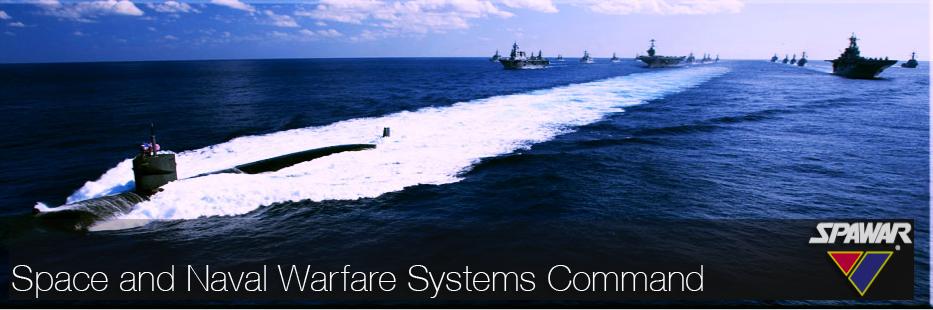
\includegraphics[scale=.4]{figures/bannerOverlay.png}
  \end{figure}
\pause \textit{`No problem. Vielen Dank  for the reply.'}
\end{block}
\pause
 \begin{itemize}
   \item Many reports from academic institutes. In general, no need to blacklist.
   \item $<10$ wanted to be blacklisted -- 50\% of them private persons.
 \end{itemize}
\end{frame}



\begin{frame}
\frametitle{Our position}
  \begin{block}{A first step towards gathering better data}
    \begin{itemize}
       \item We \textit{do not} advertise Crossbear as a silver bullet
       \item Best results can be expected against the non-selective attacker
       \item These are also the attackers we are most interested in
     \end{itemize}
  \end{block}
  \begin{block}{Crossbear is deployed and ready}
    \begin{itemize}
      \item 150 hunters on PlanetLab
      \item 4,000 certificate reports -- no MitM
    \end{itemize}  
  \end{block}
\end{frame}

